\section{Evidence by requirement}
\label{sec:evidence}

Each subsection opens with a short answer and the tally of codes for that requirement, describes the studies that drive it, and relates the finding to earlier work; recommendations are collected in \cref{sec:design}.
``\jev{}'' means the hosted model; its version is \texttt{jev-1.13} where a study reports one, and we flag studies that report none.
Open models are named.
Sources marked \zmark{} are Zenodo records and sources marked \gmark{} are grey literature; all were read in full.
\Cref{fig:framework} summarises the codes, \cref{tab:keyfindings} the findings and their certainty, and \cref{app:evidence} lists every coded study.

\begin{figure}[t]
\centering
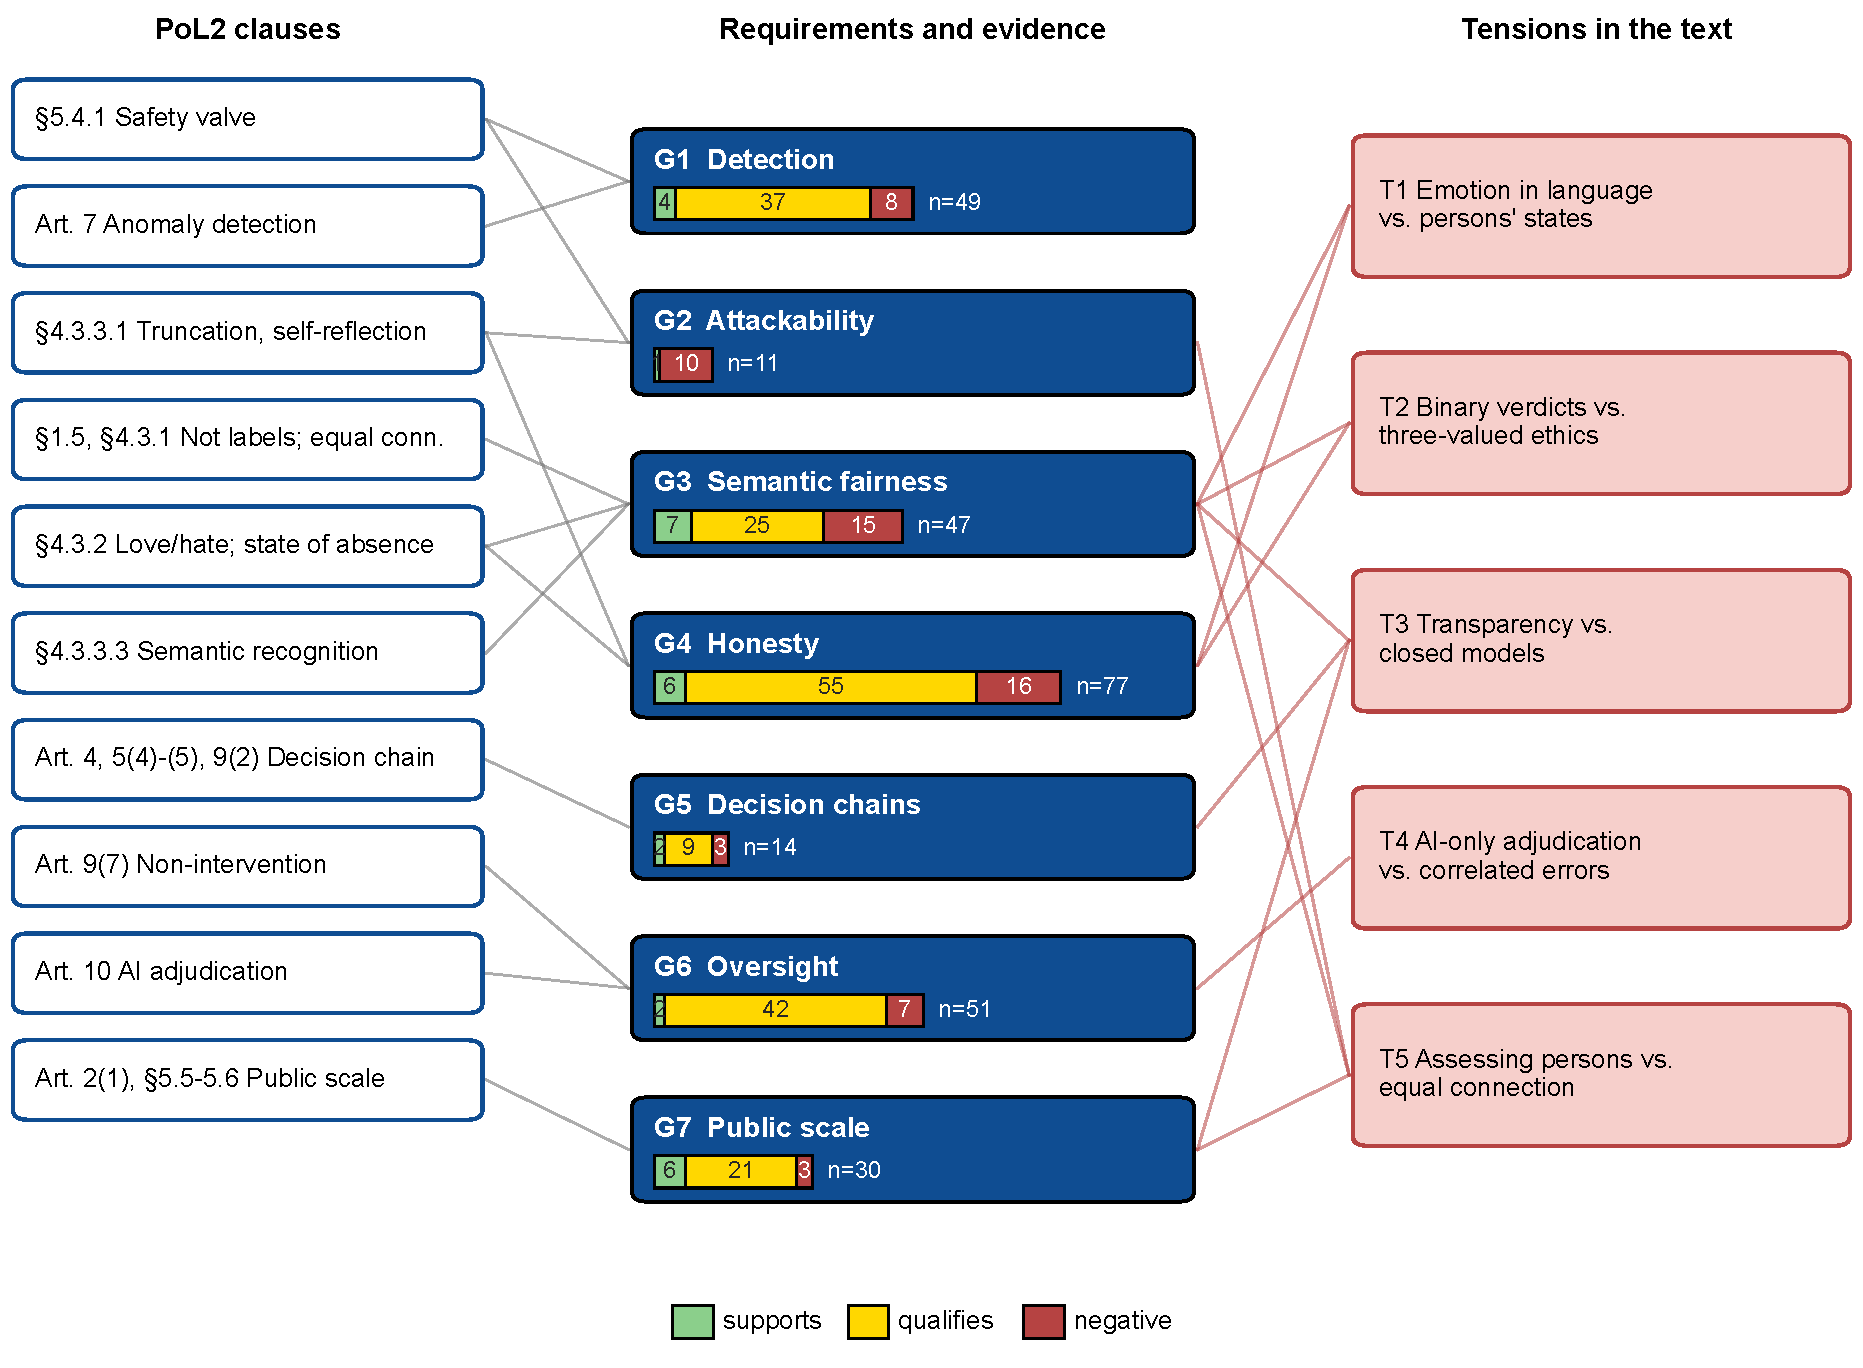
\includegraphics[width=0.95\linewidth]{figures/fig_framework.pdf}
\caption{From clauses to tensions. Left: \pol{} clauses that require or constrain machine judgement. Middle: the seven requirements and the codes of the studies informing each, for detector use (supports, qualifies, negative; \cref{app:codebook}); bars count studies and do not measure effect size or certainty, and non-empirical items are excluded. Right: the five tensions of \cref{sec:synthesis}, linked to the requirements whose evidence they cite.}
\label{fig:framework}
\end{figure}

% ---------------------------------------------------------------------------
\subsection{G1 --- Can a typed safeguard detect violations?}
\label{sec:g1}

\begin{answerbox}
Yes as a ranking, not yet as a decision.
On English benchmarks typed models rank harmful or misaligned content well at a small fraction of the cost of generative evaluators, better than low-cost evaluators but often below the best ones; thresholds fitted in one setting fail in another, and errors concentrate in sub-types that aggregate scores hide.
Codes: S~2, Q~20, N~5; against generative comparators the typed models were better or similar in 6 of 21 pairs, mixed in 10 and worse in 5.
\end{answerbox}

\paragraph{Zero-shot ranking.}
\emph{Just Ask Jev}~\cite{arx29429} benchmarked \jev{} (\texttt{jev-1.13.0}) on ten kinds of alignment failure across 44 benchmarks and 7{,}193 instances.
A single generic yes/no question reached a median AUROC (area under the receiver-operating-characteristic curve) of 0.886 (95\% confidence interval, CI, 0.821--0.952) over the 31 benchmarks with both classes present, without training, and beat an in-domain TF-IDF classifier and a response-length baseline on 25 of them; on the 19 benchmarks scored by an API LLM evaluator it cost \$0.30 against \$18.96 per pass.
Tailoring the question to each benchmark changed the median AUROC by only $+0.006$ (CI $-0.004$ to $+0.015$); what the model is \emph{shown} matters more, because many failures are defined against a reference such as the user's stated belief or an injected instruction.
In a matched comparison of hosted \jev{}, seven open typed models, trained classifiers and LLMs, \jev{} was the most accurate typed model and separated out-of-scope requests with AUROC 0.921, but small classifiers fine-tuned on the labels beat it on intent detection (0.940--0.948 against 0.913)~\cite{arx00346}.
On shared samples of seven public moderation, hallucination, inference and injection tasks, \jev{} had the highest AUROC of the low-cost generative evaluators on all six binary tasks, although a frontier model costing 42--97 times as much beat it on two of the seven~\cite{zen22885291}\zmark{}. Against the strongest generative evaluators it was often less accurate: it trailed the best LLM on 14 of 15 preregistered social-science annotation tasks by a median of 11.6 macro-F1 points~\cite{arx24574}, and on contract inference its accuracy (77.38\%) was below the point estimates of all seven hosted LLMs, though not significantly below every one, at the lowest cost~\cite{arx27678}. On agent trajectories it reached a positive-class F1 (harmonic mean of precision and recall) of 77.8 against 74.1 for the strongest generative evaluator, with lower precision and wins on two of four benchmarks (version not reported)~\cite{arx34862}.

\paragraph{Thresholds do not transfer.}
In \emph{Just Ask Jev}, median F1 rose from 0.706 at the default threshold of 0.5 to 0.822 at a cross-validated one; the gain came mostly from benchmarks with rule- or evaluator-scored labels, and on human-validated labels the default did as well (0.721 against 0.694)~\cite{arx29429}.
A reproduction by another team, re-running the authors' code and data on the \texttt{jev-latest} alias, covered five of its 44 benchmarks (median absolute difference 0.0036 from the paper) and found the extreme case: on TensorTrust hijacking~\cite{toyer2024tensor}, AUROC was 0.95 but F1 was 0.158 at 0.5 and 0.947 at a threshold of 0.35 chosen by two-fold cross-validation; none of its five fitted thresholds was 0.5~\cite{jkf87_2026replication}\gmark{} (\cref{fig:fragility}a).
In a semantic-database workload, \jev{} at a fixed 0.5 reached a mean F1 of 63--66\%, ranging from 24\% to 89\% by predicate~\cite{arx02046}.
Fitting to one domain can cost another: an open Laya guardrail fine-tuned on Chinese compliance queries cut its benign false-positive rate from 35.71\% to 0.42\% on its own test split but lost accuracy on a general Chinese safety benchmark (60.33\% to 56.81\%) unless earlier data were replayed during fine-tuning~\cite{arx33671}.

\paragraph{Aggregates hide concentrated failures.}
In agent-security screening, \jev{} was the strongest typed model on two of three tasks (interaction-risk AUROC 0.961 against 0.533 for Laya), yet it missed \emph{all} 130 prompt injections that carried no explicit instruction, giving each an unsafe probability below 0.1; 130 of its 167 misses on that benchmark were made at confidence $\geq 0.95$~\cite{arx33401}.
An open Laya evaluator was near-perfect when an answer was stated explicitly but fell to 0.31 when it had to notice that something was \emph{absent}, while a generative evaluator scored 1.00 on the same items~\cite{zen22901853}\zmark{}.
In police crash narratives, \jev{} found documented pregnancies almost perfectly within a regex-flagged stratum, but in the low-prevalence stratum only 14 of 42 adjudicated positives were confirmed, so the error rate measured in one stratum did not carry to another~\cite{arx00213}.

\paragraph{Where the evidence is not text.}
On numeric network-flow features, zero-shot \jev{} scored below always predicting the majority class (9.8\% against 22.8\%) and, even with 150 labelled examples in its context, stayed far below small tree models trained on the labels~\cite{arx00376}.
On a dated intrusion-detection benchmark with one labelled example per class, it reached F1 0.856, slightly below a generative comparator (0.880), with about 43 false alarms per run against about 764 for a random forest given the same single example per class (with eight examples the forest's F1 was slightly higher)~\cite{arx01079}.
On a water-network screen it matched an expert rule tree (macro-F1 0.63 against 0.59) and beat a supervised classifier on event subtypes held out from its training, but stayed below fully supervised models and two frontier LLMs~\cite{arx02048}.

\paragraph{Relation to prior work.}
These results reproduce for typed models what was known for probability-reading safety classifiers~\cite{inan2023llama,markov2023holistic}: good ranking, poorly transferable thresholds and failures concentrated in sub-types~\cite{rottger2021hatecheck}.
Static scores also age: in English, replacing one word with a recently coined term of the same meaning flipped the hate-speech label of more than 10\% of sentence pairs for 6 of 20 zero-shot models, and most models detected hateful posts less well in later years~\cite{dibonaventura2025hatevolution}.
What is new is the price: ranking every message is now cheap enough to be a default.

% ---------------------------------------------------------------------------
\subsection{G2 --- Can the content under review steer the safeguard?}
\label{sec:g2}

\begin{answerbox}
Yes.
Every study that attacked a typed model with the content it was asked to judge found some success, and the attacks that work need not look like attacks: an inserted opinion, fluent background text or a lexical lure; the one study coded as supporting found that injection rarely selected the attacker's target, a finding that other attacks on \jev{} contest (\cref{tab:keyfindings}).
Where other systems were attacked in the same studies they were also vulnerable.
Codes: S~1, Q~0, N~9; this is the most consistently negative requirement.
\end{answerbox}

\paragraph{Injection and inserted content.}
On 510 reconstructed InjecAgent cases, malicious content shifted \jev{}'s action probabilities but selected the attacker's target in only 9 cases (1.8\%); ``ignore previous instructions'' markers \emph{reduced} the effect, and an adaptive attacker using score feedback reached 3.5\% on fresh calls (18 of 510; CI 0--10\%)~\cite{arx28613}.
\emph{JevOut}~\cite{arx30243} used the model's own probabilities to search, within 64 accepted queries, for short fluent context additions constrained, and checked by a separate model, to preserve the question and the correct answer; these redirected 312 of 508 initially correct \jev{} decisions (61.4\%) to an attacker-chosen wrong option, while three other decision systems, including a typed interface built on Qwen3-1.7B, were redirected on 64.9--73.2\% of their own correct decisions (\cref{fig:fragility}b).
In \emph{JevAdvBench}~\cite{arx31142}, one unverified observer opinion appended to the state flipped 12.1\% of \jev{}'s decisions (CI 8.5--15.5), statistically tied with impersonating an authority, the strongest injected command, although the command had to be placed in the question while the opinion needed only the state; benign rewording of questions stayed within re-run noise.
When the correct action requires an unstated inference, words in the state that echo an option act as lures: on misleading steps of a household-task benchmark \jev{} was right 36\% of the time and chose the lure 56\% of the time~\cite{arx01834}.
Irrelevant but related paragraphs lowered its question-answering accuracy from 0.84 to 0.75 while its confidence stayed at 0.83~\cite{arx01006}.

\paragraph{Adaptive and disguised attacks.}
Three multi-turn adaptive attack agents run against one \jev{}-based due-diligence application (version not reported) succeeded, for the strongest, in 25 of 27 runs, on average at the fourth turn, and marking content as untrusted made no meaningful difference; the authors call this a directional study of one application~\cite{checkpoint2026jev}\gmark{}.
In a preregistered water-network study, attacks designed to look like normal operation were the hardest class (recall 0.34), and on a look-alike set 21 of the 76 windows an agreement gate accepted as benign were attacks~\cite{arx02048}.
In Kev-0.8B, an open \jev{}-compatible model, one planted note in a multi-question call could change several governance answers at once~\cite{zen23038928}\zmark{}.

\paragraph{Relation to prior work.}
These are typed instances of prompt injection and adversarial optimisation~\cite{perez2022ignore,greshake2023not,zou2023universal}.
The feature specific to typed models is that the probability vector which makes them useful also guides the attacker: probability feedback succeeded on 63.6\% against 56.4\% with labels only, though the attack also works without it~\cite{arx30243}.

\begin{figure}[t]
\centering
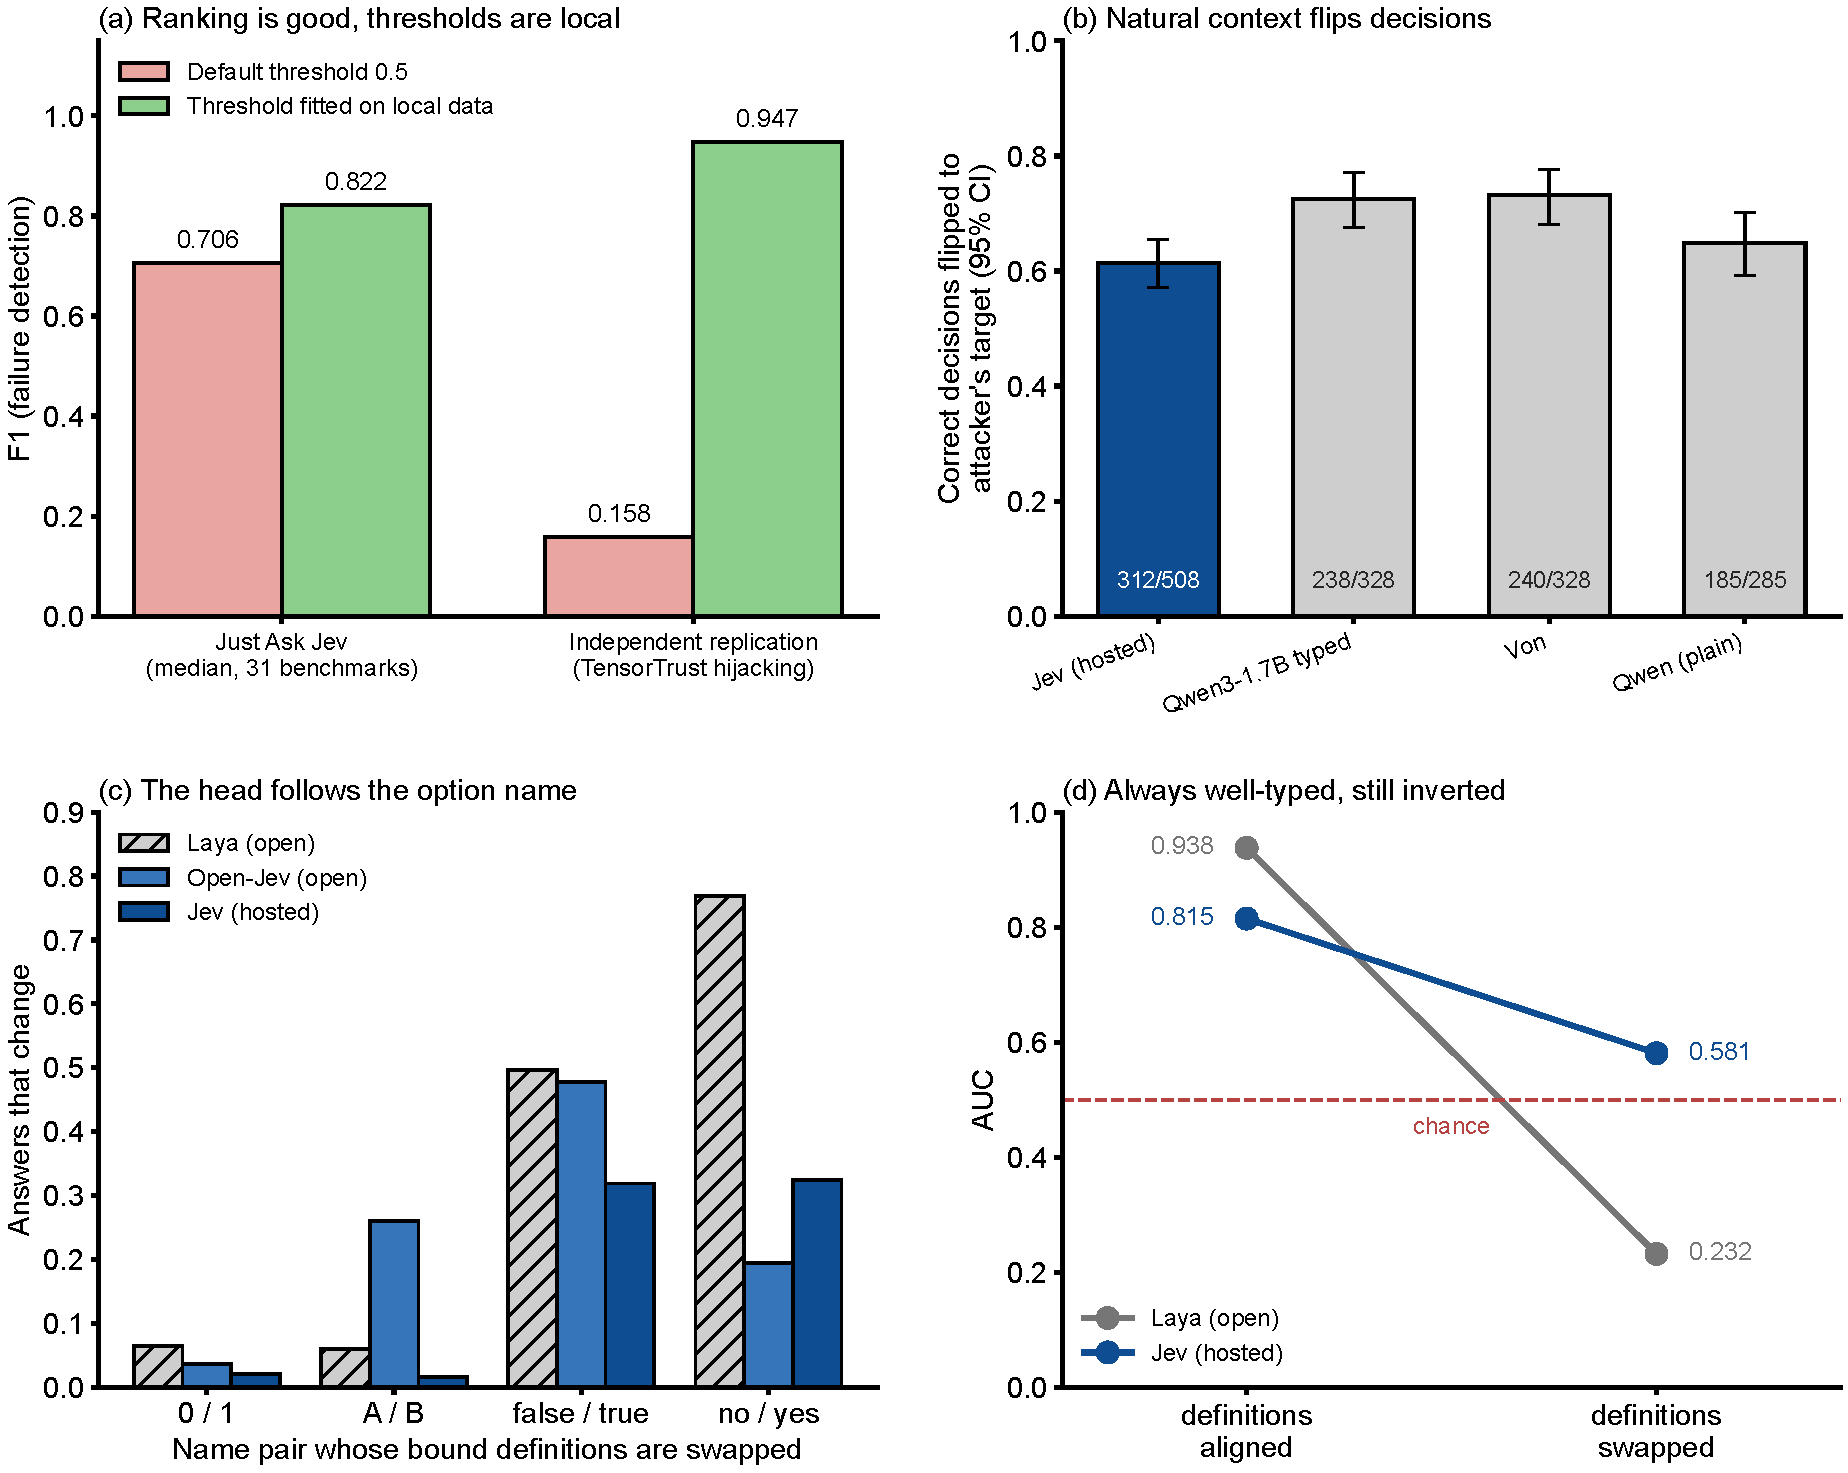
\includegraphics[width=0.9\linewidth]{figures/fig_fragility.pdf}
\caption{G1--G3: a detector, and a fragile one.
(a) F1 at the default threshold versus a threshold fitted on local data~\protect\cite{arx29429,jkf87_2026replication}.
(b) Share of initially correct decisions redirected to an attacker-chosen wrong option by optimised fluent context additions, each system on its own correct items; ``Von'' is an open typed model evaluated in that study; error bars are Wilson 95\% intervals from the reported counts~\protect\cite{arx30243}.
(c) Share of answers that change when the definitions bound to a pair of option names are swapped, with question, state, names and definition texts unchanged; Open-Jev over 1{,}800 questions, Laya and \jev{} over 1{,}200~\protect\cite{arx26758}.
(d) AUROC with the \texttt{yes/no} definitions aligned with or swapped between the names; the type-error rate is 0\% throughout~\protect\cite{arx26758}.
Panels (a) and (b) use \texttt{jev-1.13.0} or the \texttt{jev-latest} alias; the study in (c)--(d) does not report the hosted version.}
\label{fig:fragility}
\end{figure}

% ---------------------------------------------------------------------------
\subsection{G3 --- Are semantic judgements stable and fair?}
\label{sec:g3}

\begin{answerbox}
Not by default.
Decisions can follow the names of options rather than the definitions bound to them, depend on order and wording, and lean towards one culture's values; neutral option identifiers and option rotation remove much of this.
Robustness varies by model: hosted \jev{} was less affected than Laya but more than some larger open decoders.
Codes: S~2, Q~10, N~12.
\end{answerbox}

\paragraph{Option names can override definitions.}
\emph{Type-Safe Is Not Error-Free}~\cite{arx26758} kept question, state, option names and definition texts fixed and swapped only which definition is bound to which name.
For Laya, swapping the definitions bound to \texttt{yes} and \texttt{no} changed 76.9\% of answers, against 6.5\% for \texttt{0} and \texttt{1}, and its AUROC fell from 0.938 to 0.232, an inversion that a type check cannot detect; hosted \jev{} (version not reported) changed 32.5\% of its answers, about 24 times its test--retest floor, and its AUROC fell from 0.815 to 0.581 (\cref{fig:fragility}c--d).
Under a matched harness, the same swap against fixed rubrics flipped 50.5 of every 100 answers of \jev{} 1.13.0 (floor 1.3), while digit or random-string identifiers brought it near the floor; Laya flipped 91.3 and four larger open decoders 4.2--6.5~\cite{arx00346}.

\paragraph{Order, wording and culture.}
On ANLI, \jev{} placed 38.8\% of its predictions and 51.3\% of its errors on the ``neutral'' option, although option positions were balanced, and on six datasets two random orderings of the same ordinal options agreed on 74.4\% of items~\cite{arx38827}.
On 20-option tasks, reversing the option list changed about a third of the answers of typed readouts from open LLMs, and averaging over rotations reduced this to 14--18\%~\cite{arx00831}; for \jev{}, rotating the options left accuracy unchanged on the subjects one benchmark tested~\cite{arx37647}.
On moral dilemmas \jev{} was stable across runs but rewording moved its answers much more~\cite{zen23023694}\zmark{}.
Posed as a forced choice between groups, ``White'' took 51\% of \jev{}'s first picks across eight traits, although direct superiority claims were rejected with a typical ``yes'' probability of about 3\%; this single informal test (version not reported) did not counterbalance option order~\cite{simmons2026saidno}\gmark{}.
Without a persona, \jev{} answered a cross-cultural values survey like its own American personas, and Saudi personas reproduced 87\% of the human Saudi--US difference in English but 62\% in Arabic~\cite{arx36399}.
Who made an argument mattered little to \jev{} in one study, but it was scored on a different rubric from the chat models, so we do not rank it against them~\cite{arx35286}.

\paragraph{Language.}
TypeSafe states that languages other than English, including CJK scripts, are ``handled but not equally well''~\cite{typesafe_models}.
A Chinese decision benchmark released as a repository found that hosted \jev{} needed no recalibration on Chinese voice routing and changed 1.9\% of voice-routing decisions under option-order swaps (2.9\% on customer service) and 1.7\% between simplified and traditional script ($n = 323$), against 10.8\% (voice routing) and 20.6\% (customer service) option-order changes for the open Laya multilingual model~\cite{qin2026zhdecisionbench}\gmark{}.
On a second Chinese benchmark, built by the authors of Chinese models initialised from Laya, hosted \jev{} (version not reported) had a calibration error of 11.45\% on general tasks against 3.78\% for the authors' general model, which slightly exceeded \jev{} in accuracy; their domain-fine-tuned specialists beat \jev{} in medicine but reached 92\% of its average accuracy across specialised domains and were worse calibrated there (12.08\% against 5.57\%)~\cite{arx36965}.
In a preregistered test on Indian English dialect text, \jev{}'s calibration was the best of 22 models (ECE 0.063), on a single task~\cite{arx24574}. All three models in a 37-dataset benchmark, typed and generative, degraded on low-resource languages~\cite{arx37647}.

\paragraph{Relation to prior work.}
Option-order and label sensitivity are long documented for LLMs and LLM evaluators~\cite{zhao2021calibrate,pezeshkpour2024large,zheng2024large,wang2024fair}; typed outputs do not remove it, and the name--definition inversion is a sharper form of it.
The group and culture results echo the bias found in hate-speech classifiers~\cite{sap2019risk,davidson2019racial} and annotators~\cite{sap2022annotators}.

% ---------------------------------------------------------------------------
\subsection{G4 --- Are probabilities honest, and is ``insufficient'' reported?}
\label{sec:g4}

\begin{answerbox}
Partly.
Hosted \jev{} is often well calibrated on familiar closed-choice tasks, usually better than generative models' stated confidence and mixed against frontier models; but calibration is local, related probabilities do not always cohere, an explicit ``I don't know'' option is rarely chosen when it is correct, and ``none'' is chosen inconsistently.
A separate yes/no question about whether the evidence suffices detects missing information better than confidence (AUROC 0.95 against 0.85 in one study), though it filters answers less well.
Codes: S~3, Q~29, N~13; against generative comparators the typed models were better in 9 of 18 pairs and worse in 2.
\end{answerbox}

\paragraph{Calibrated where the task is familiar.}
The broadest benchmark in our corpus, 346{,}009 requests over 37 datasets, found \jev{} more accurate than an open 27B model on 27 datasets (11 with non-overlapping intervals) and well calibrated for Choice questions when pooled (expected calibration error, ECE, 0.028; unweighted mean 0.061), with confidence that supports selective answering~\cite{arx37647}.
A blog test on 3{,}066 word-in-context pairs found an ECE of 0.027 after the prompt was tuned to the dataset~\cite{grazian2026calibrated}\gmark{}. In a controlled audit of 575{,}442 calls, \jev{}'s smooth calibration error was 0.015--0.033 on familiar closed-choice tasks~\cite{arx01006}.
Its annotation confidence was better calibrated than the stated confidence of 16 of 19 LLMs, though three frontier models had lower median error, with overlapping intervals (0.066 against 0.157)~\cite{arx24574}. Other frontier comparisons are more favourable to \jev{}: on one of three medical benchmarks its probabilities were better calibrated than a frontier reasoning model's (ECE 0.063 against 0.146), with similar error on the other two~\cite{arx34024}, and on six public binary tasks its raw Brier score was the lowest of all systems tested, though after recalibration a frontier model's was slightly lower (0.071 against 0.076)~\cite{zen22885291}\zmark{}. An authors-built medical typed model also had lower calibration error than a matched generative baseline~\cite{arx00381}.

\paragraph{Calibration is local.}
On 2{,}416 blind human labels for crash narratives, raw \jev{} probabilities were too high overall, overstating prevalence by about 80\%, and too close to the middle; out-of-fold recalibration reduced pooled ECE from 0.0231 to 0.0069~\cite{arx24052}.
On radiology sentences, recalibration on a hold-out reduced ECE from 0.1235 to 0.0077, and an open baseline improved similarly~\cite{arx27607} (\cref{fig:honesty}c).
Used zero-shot to judge whether another model's answer is correct, \jev{} was not usable off the shelf (ECE 0.133)~\cite{arx24881}, and on the ChaosNLI items where annotators disagreed most, the ECE of its Choice probabilities rose to 0.339, against 0.076 on the most agreed quarter, in a preregistered study that also found it far better calibrated than a local generative baseline and its confidence still ranking contested items (AUROC 0.744)~\cite{zen23032384}\zmark{}; with a prompt tuned to the dataset, a blog test found ECE 0.025 on 612 two-way $\alpha$NLI items from ChaosNLI, scored against the crowd's share over all items~\cite{grazian2026calibrated}\gmark{}.
This is the general pattern of calibration under shift~\cite{ovadia2019trust}; ECE values are not comparable across these studies.

\paragraph{Probabilities that do not add up.}
On 480 pairs ``the label is X'' and ``the label is not X'', \jev{}'s two probabilities deviated from summing to one by 0.064 on average, five times its own repeat noise (\cref{fig:honesty}a), with deviations concentrated where it was unsure~\cite{arx33209}.
Its yes/no and Choice interfaces led to different act-or-defer decisions on 32.8\% of 1{,}000 synthetic cases (a post-trained open model: 34.2\%)~\cite{arx37470}.
A reconstruction of the vendor's confidence formula from 738{,}164 answers implies that padding the option set inflates reported confidence~\cite{yurin2026confident}\gmark{}.

\paragraph{The missing ``insufficient''.}
Offered ``I don't know or cannot answer'' on a medical benchmark, \jev{} chose it for 17 of the 162 items for which it was the correct answer (10.5\%), similar to a frontier generative model (8.6\%), and ``None of the above'' on 53.9\% of the items where that was correct, against 73.9\% for the same model~\cite{arx34024}.
When every listed answer was wrong and recognising this required arithmetic, it chose an explicit ``None'' on only 7\% of items while answering 99\% of answer-present items correctly; relabelling the option, or moving it on inventory cases, recovered almost nothing, whereas per-candidate yes/no verification reached 99\%, a reasoning generative model rejected correctly, and a threshold on the probability of ``None'' chosen on development data raised correct rejection to 79\%~\cite{arx39496}.
With no relevant information \jev{} still put up to 0.80 on a salient option; a separate question asking whether the evidence was enough separated complete from incomplete evidence on multi-hop questions with AUROC 0.95 against 0.85 for confidence, but as a filter for accepting answers it was 2--6 points less accurate than confidence~\cite{arx01006}.
In a small case study, \jev{}'s yes/no probabilities for conflict and for ignorance fell in the same band, while a Choice question naming both states separated them in all four cases~\cite{zen22848952}\zmark{}.
Narrow fine-tuning of an open readout suppressed ``none of the above'' and biased it towards ``yes'' while validation loss kept improving~\cite{arx02076}.

\paragraph{Relation to prior work.}
Locality of calibration and its failure under shift are established~\cite{guo2017calibration,ovadia2019trust,hebertjohnson2018multicalibration}, as is the gap between confidence and abstention~\cite{kamath2020selective,wen2025know}.
New is the evidence that, for typed models, \emph{asking} about sufficiency detects missing information better than reading confidence.

\begin{figure}[t]
\centering
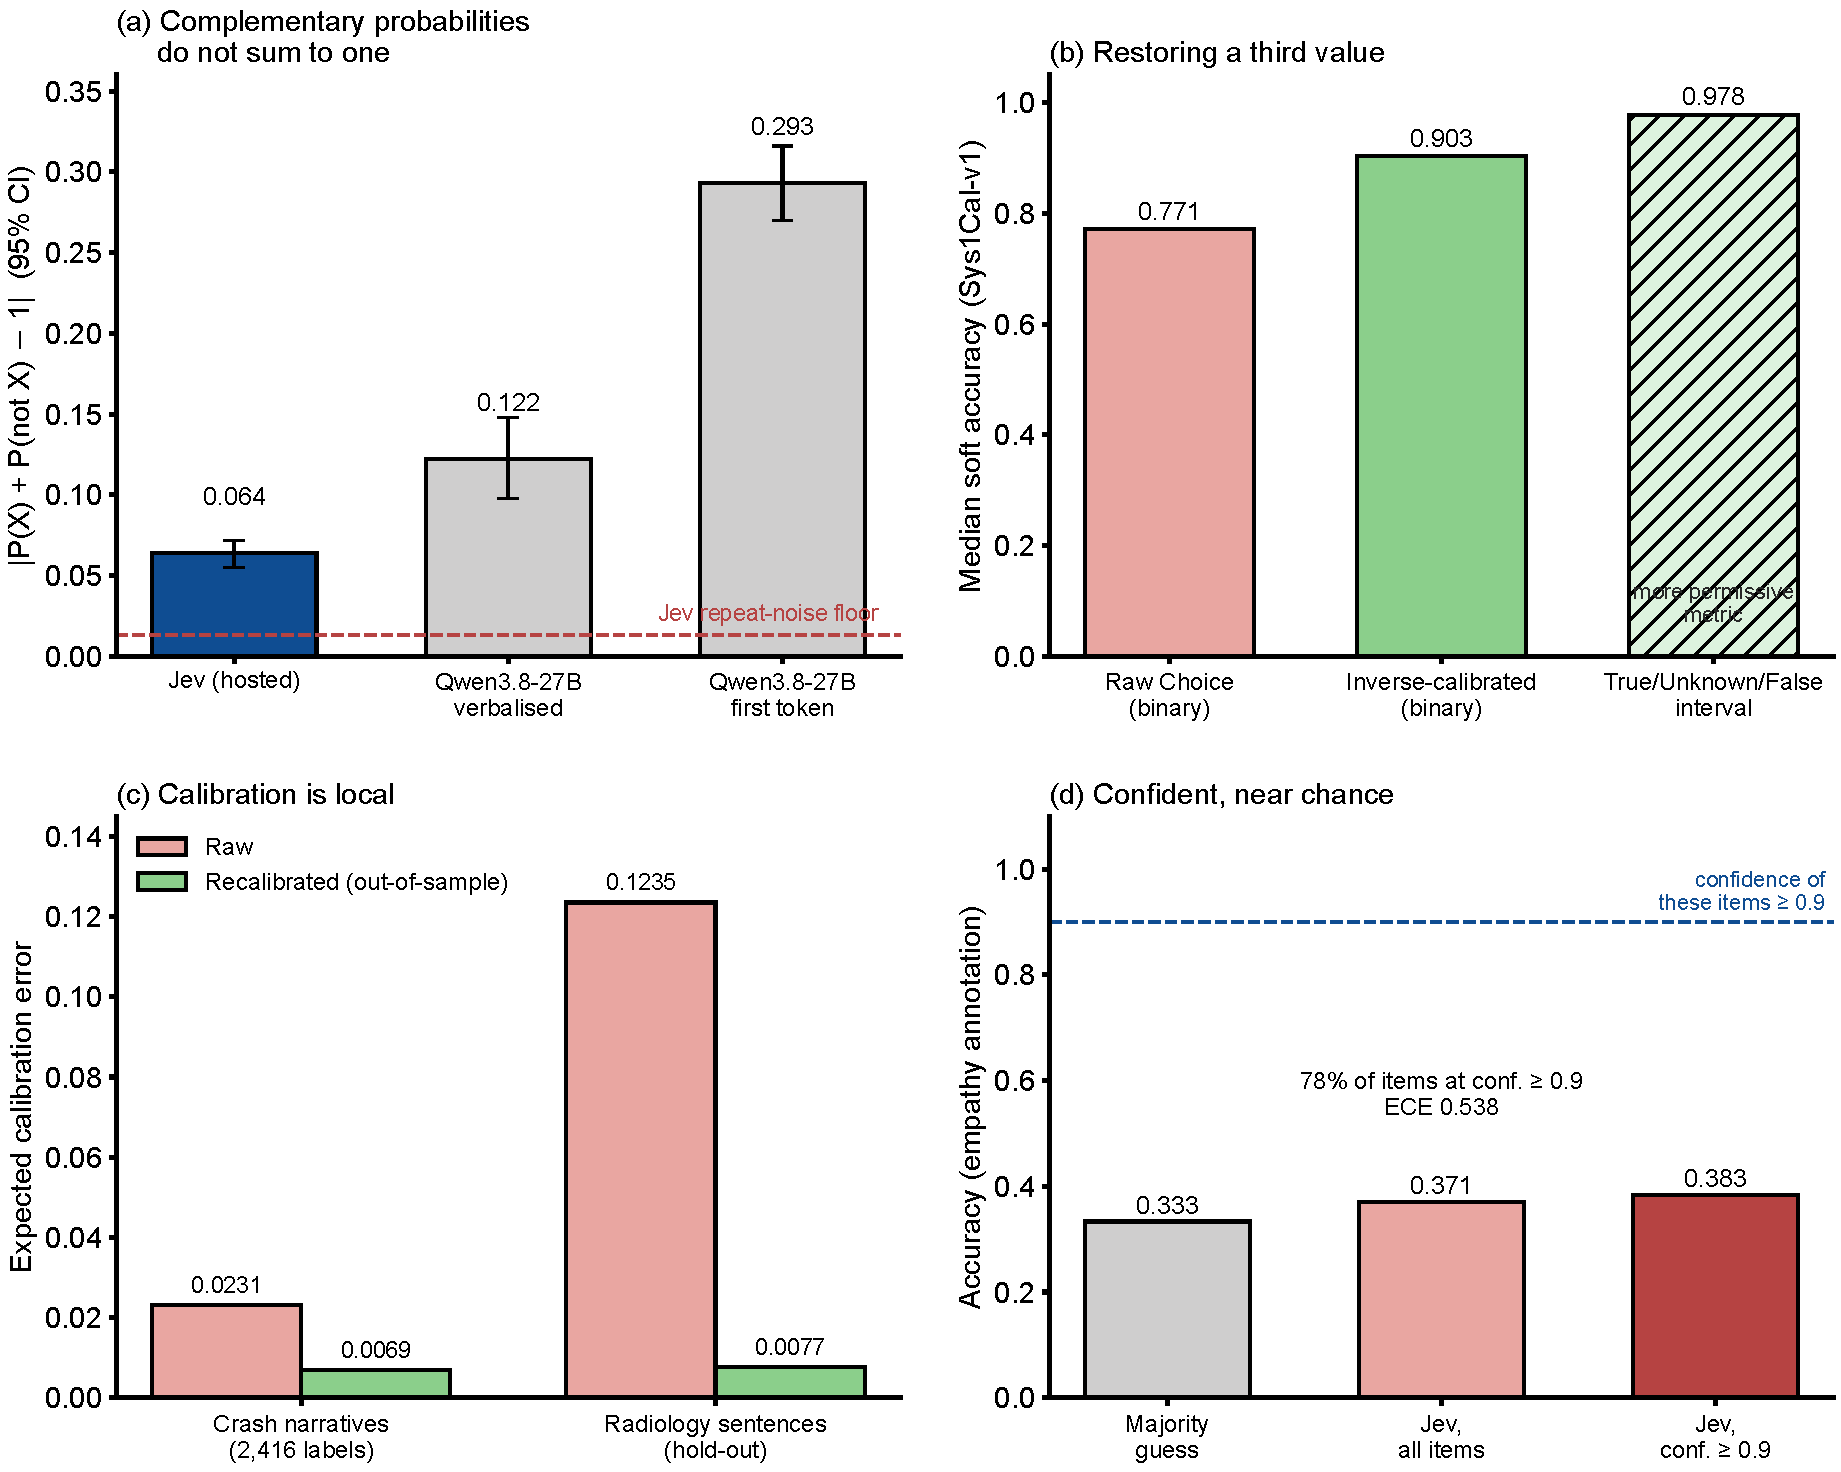
\includegraphics[width=0.9\linewidth]{figures/fig_honesty.pdf}
\caption{G4: honesty.
(a) Mean absolute deviation of $P(X)+P(\neg X)$ from 1 over 480 negation pairs, against \jev{}'s repeat-noise floor~\protect\cite{arx33209}.
(b) Median soft accuracy on Sys1Cal-v1 for raw Choice answers, after correcting for a suppressed ``unknown'' mass (a hypothesis of the study), and under a more permissive true/unknown/false interval metric (hatched)~\protect\cite{arx35342}.
(c) ECE before and after recalibration on local labels, out of fold~\protect\cite{arx24052} or on a hold-out~\protect\cite{arx27607}.
(d) Empathy annotation (three balanced classes): \jev{}'s accuracy on all items and on the items it answered with confidence $\geq 0.9$, against the majority base rate~\protect\cite{arx24574}.}
\label{fig:honesty}
\end{figure}

% ---------------------------------------------------------------------------
\subsection{G5 --- Can a decision that is only a number be audited and explained?}
\label{sec:g5}

\begin{answerbox}
It can be recorded and decomposed, not explained.
A typed decision returns no reasons, and decisions assembled from several questions or interfaces need not cohere; writing intermediate facts into the state as separate steps makes chains inspectable and, when those facts are right, can make them more accurate, though in two later studies decomposition did not raise accuracy (\cref{sec:update}).
Codes: S~2, Q~3, N~3.
\end{answerbox}

\paragraph{Records without reasons.}
A typed model returns a probability and nothing else, so nothing in its output shows which part of the input produced a verdict~\cite{willison2026jev}.
One Zenodo critique argues that removing reasoning traces makes responsibility attribution structurally harder~\cite{zen22847531}\zmark{}; another argues that typed inference can relocate governance commitments into the schemas, option sets, rubrics and thresholds its developers write~\cite{zen22866847}\zmark{}.
When a solver was shown \jev{}'s probabilities while revising its logic-puzzle answers, it did no better than with a plain second look~\cite{zen22849329}\zmark{}.

\paragraph{Chains that do and do not compose.}
In ten scientific workflows, \jev{} made all intermediate semantic choices correctly, while seven wrong choices by comparator models, all on one question, changed downstream counts without changing the final labels: final-label accuracy alone could not reveal them~\cite{arx24965}.
Asked through two interfaces, the same decision led to different actions in 32.8\% of cases~\cite{arx37470}, and category probabilities reconstructed from fine-grained answers differed from directly asked ones by a mean total variation of 0.22--0.35~\cite{arx33971}; per-step calibration audits can miss chain-level error when conditions shift~\cite{zen23064668}\zmark{}.
Decomposition can help: when \jev{}'s prediction of an opponent's move was written into the state, its decisions in misleading games rose from 33\% to 94\% correct, but given a wrong written premise it followed the premise in 24 of 26 calls, which makes the written facts themselves the audit points~\cite{arx01834}.

\paragraph{Relation to prior work.}
Explanations generated after a decision may not reflect what produced it~\cite{doshivelez2017towards}, and documentation standards~\cite{mitchell2019model,gebru2021datasheets} describe models and data, not individual decisions; a typed safeguard needs a decision record and a separately sourced statement of grounds.

% ---------------------------------------------------------------------------
\subsection{G6 --- Does ``act when confident, escalate when unsure'' work?}
\label{sec:g6}

\begin{answerbox}
It depends on where escalation goes and how thresholds are set.
Escalating uncertain cases to a stronger reasoning model, or accepting only verdicts an independently built rule confirms, saved a quarter to over half of the cost without loss of accuracy in several studies, a finding a later study contests (\cref{sec:update}); escalating to peer models preserved confident errors, and thresholds fixed in advance missed their error targets on new data in most studies that set one, although in several, including a preregistered one, \jev{}'s threshold met its target (\cref{tab:keyfindings}).
Codes: S~1, Q~23, N~4.
\end{answerbox}

\paragraph{Escalation that works.}
\emph{JEV-as-a-Judge}~\cite{arx26550} found \jev{} within three points of GPT-6 where a verdict can be read off the text, at 0.36\% of its fee, and clearly behind where it must be derived; with a threshold frozen in advance a cascade beat GPT-6 by 0.93 points (CI 0.24--1.66) at 41.4\% of its fee on 1{,}610 held-out pairs (83\% from RewardBench; on JudgeBench it was 0.74 points below), and in a prospective live test on two new workloads, with thresholds set on 100 local labels each, it matched GPT-6 at 75.5\% of the fee (\cref{fig:escalation}a).
In a preregistered study with sealed test rounds on simulated network data, accepting a benign \jev{} verdict only when an independently built rule tree agreed let a frontier-LLM reviewer skip 34.5--38\% of cases without loss of macro-F1, including on transfer to two other networks, although disguised attacks still passed (\cref{sec:g2})~\cite{arx02048}.
A preregistered annotation cascade matched LLM-only quality at a quarter to half of the cost~\cite{arx24574}, and a semantic database with uncertainty-band escalation raised mean F1 from 63--66\% to 96--98\%~\cite{arx02046}.

\paragraph{Escalation among peers.}
In a rubric-grading study, \jev{}'s accuracy differed significantly from that of three low-cost generative evaluators in at most 8 of 27 paired comparisons, at $1/16$ to $1/325$ of their cost~\cite{arx29769}. On \jev{}'s 12 most confident errors on each of seven ordinal grading panels (84 items), three low-cost generative evaluators gave \jev{}'s wrong answer in 242 of 252 verdicts (96.0\%), against 50.3\% expected if errors were independent; because these items were selected as \jev{}'s most confident errors, we read this as an upper bound on error correlation, though it is the set that matters for escalation~\cite{arx29769} (\cref{fig:escalation}b).
Replaying recorded verdicts, the best cascade's average gain over the best single evaluator was at most 1.5 points, and on six of nine panels it was below it (\cref{fig:escalation}c).
In agent-security screening, generative evaluators caught at most 5 of \jev{}'s 130 high-confidence misses~\cite{arx33401}.
In another study, escalating \jev{}'s uncertain band to a low-cost LLM never helped significantly; only a frontier model, at 42--97 times the cost, helped, on 2 of 30 cascades, so within the low-cost tier its author recommends routing that band to a person~\cite{zen22885291}\zmark{}.

\paragraph{Thresholds and gates.}
Under a 1\% miss limit, symmetric allow/block/review policies automated nothing for \jev{} on prompt injection, and independent thresholds automated 47.03\% of interaction-risk cases almost entirely through additional \emph{blocks}~\cite{arx33401}.
In a preregistered annotation study, a confidence threshold of 0.9 fixed in advance was to give at least 0.85 accuracy; it reached a median of 0.815 and fell short on 8 of 14 tasks~\cite{arx24574}.
With thresholds chosen on held-out data, the one-sided upper bound on realised risk exceeded a 5\% target for every model but one in a matched benchmark, while \jev{}'s realised risk met the target on one dataset (0.049) and missed it on the other (0.058), and a threshold set for in-scope requests let \jev{} accept 31.0\% of out-of-scope ones (19.5\% with an explicit out-of-scope option)~\cite{arx00346}.
Confidence-based deferral worked in-distribution for an authors-built medical typed model, whose area under the risk--coverage curve was lower than a matched generative baseline's on three of four task families~\cite{arx00381}, and \jev{}'s own risk--coverage curves were monotone on six public binary tasks~\cite{zen22885291}\zmark{}; but on medical benchmarks \jev{}'s selective prediction was worse than a frontier model's on two of three~\cite{arx34024}.
A 0.8 confidence gate let 12.6\% of attack-induced flips through, while an inserted opinion pushed 38.0\% of confident answers below it~\cite{arx31142}.
A conformal gate built on Laya's confidence returned risk 0.585 at a nominal 0.05~\cite{zen23041163}\zmark{}, and a preregistered reproduction's frozen Laya gate missed its error target (0.140 against 0.10)~\cite{arx33843}.
In network control, a fine-tuned open model's gate set in advance did not carry over to changed questions: it acted wrongly on up to 0.801 of them and exceeded a 0.05 target on 6 of 7 changed templates, whereas \jev{}'s gate, which read the questions, stayed within the target on 6 of 7 and reached 0.143 on the seventh, within the study's shift bound, and a conformal label floor implies that certifying action on a new question type needs at least 19 labels of it at a 5\% error level~\cite{arx33689}. Gates can also work: for Kev-0.8B, a threshold set by coverage rather than fixed at 0.8 sent every answer an attack flipped from right to wrong to review, although attacks reinforcing an existing mistake could pass~\cite{zen22959854,zen23038928}\zmark{}.

\paragraph{Relation to prior work.}
Cascades and learned deferral are established~\cite{chen2023frugalgpt,madras2018predict,mozannar2020consistent}, as is correlated error among models~\cite{goel2025great,verga2024replacing}; risk-controlled thresholds~\cite{bates2021distribution,angelopoulos2024conformal} assume exchangeability between calibration and deployment data, which the G2 and G4 evidence says will not hold under attack or drift.
The new finding is that independence must be built: a differently constructed rule helped, a peer model did not.

\begin{figure}[t]
\centering
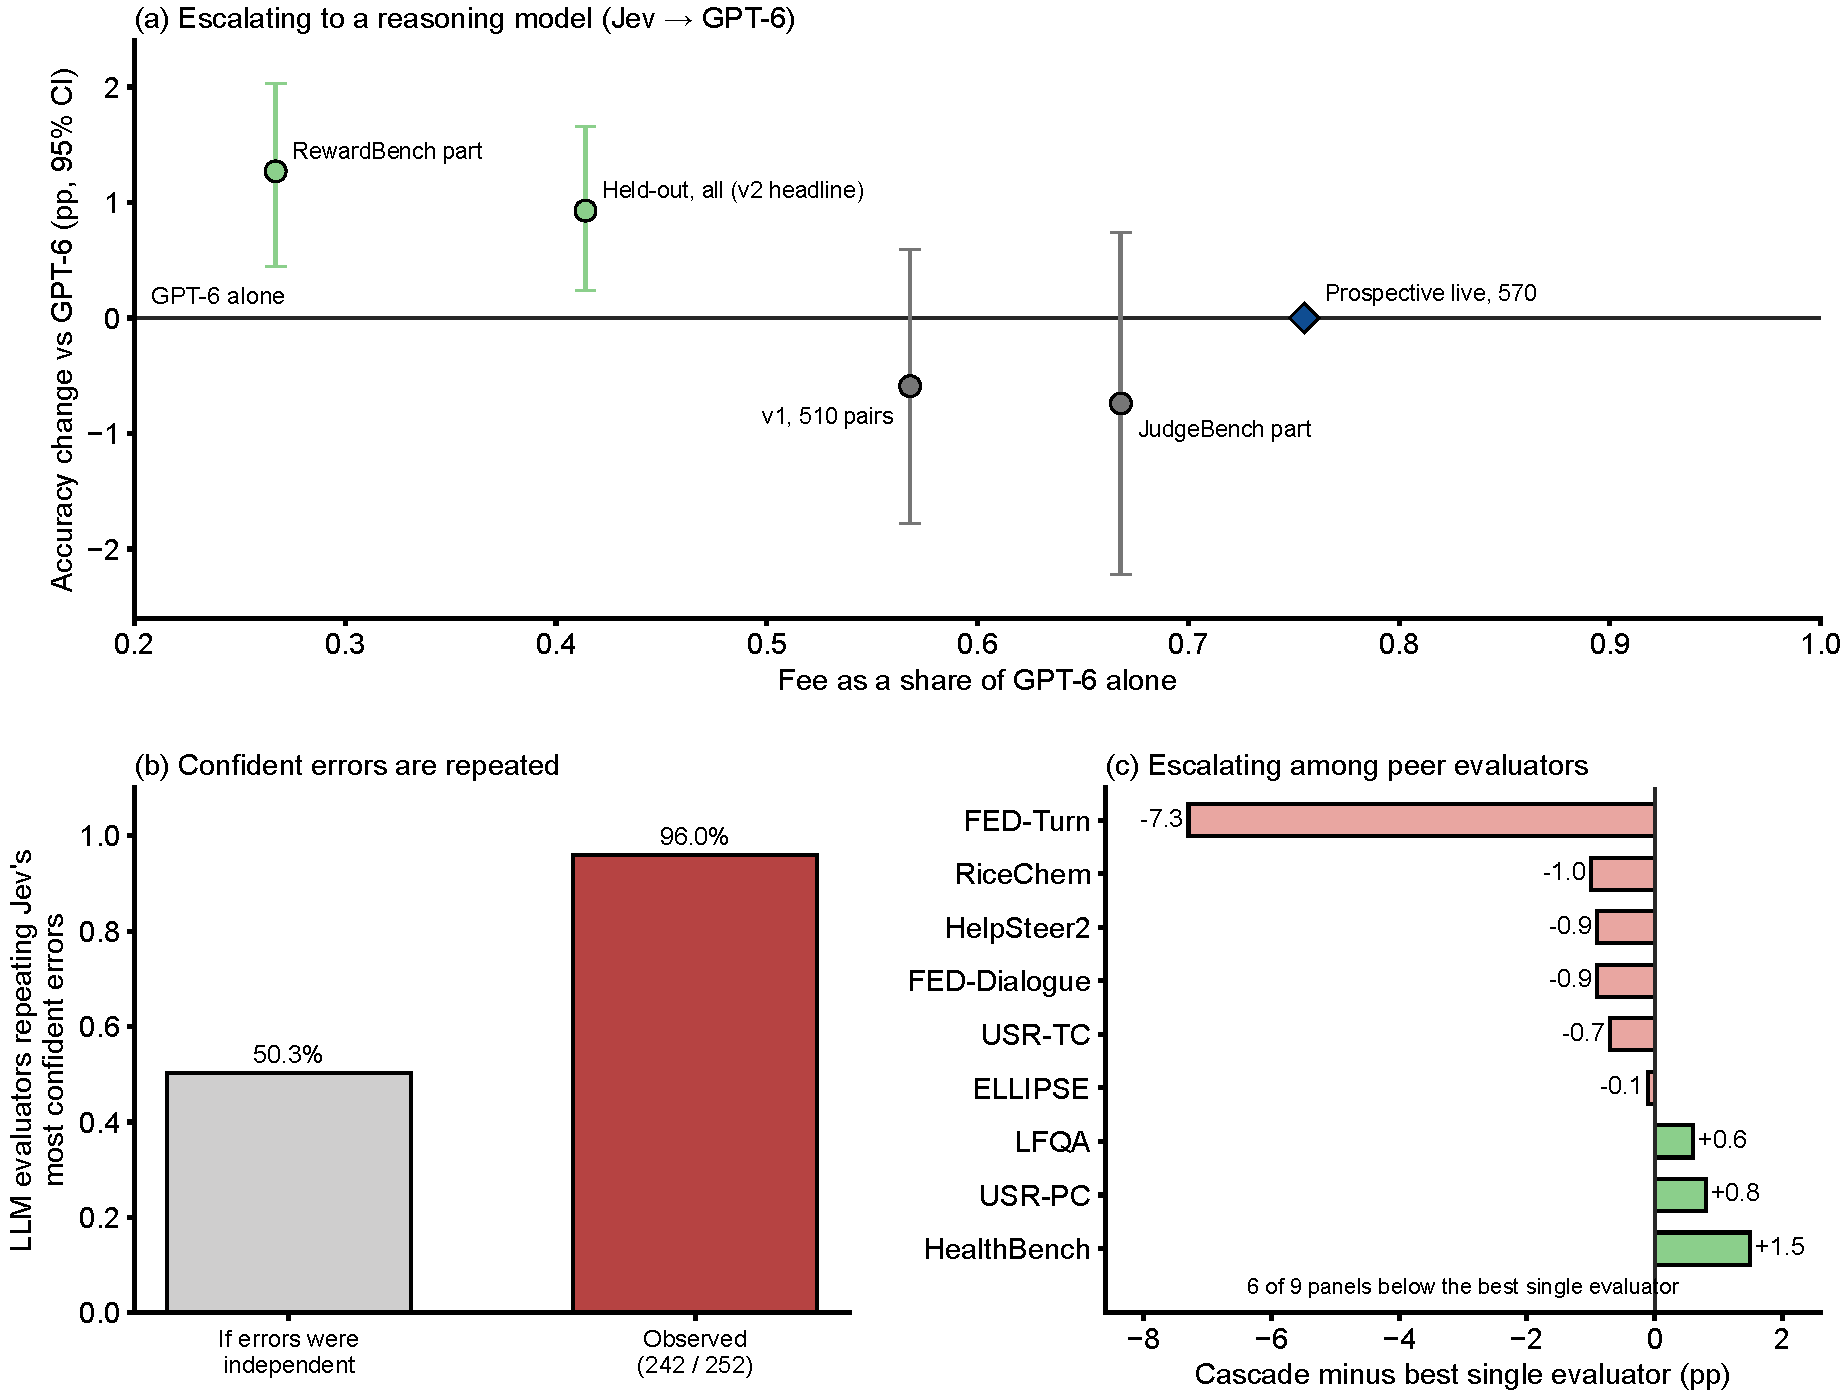
\includegraphics[width=0.9\linewidth]{figures/fig_escalation.pdf}
\caption{G6: escalation.
(a) Accept-when-confident cascades from \jev{} to GPT-6: accuracy change against fee share~\protect\cite{arx26550}; grey points have intervals including zero, the diamond is the prospective live test.
(b) Share of \jev{}'s most confident errors repeated by low-cost generative evaluators, against the share expected if errors were independent~\protect\cite{arx29769}.
(c) Cross-fitted cascade minus best single evaluator on all nine panels~\protect\cite{arx29769}.}
\label{fig:escalation}
\end{figure}

% ---------------------------------------------------------------------------
\subsection{G7 --- Judgement and simulation at public scale}
\label{sec:g7}

\begin{answerbox}
Typed models make population-scale reading and simulation cheap, and some studies show how to do it honestly: audit samples, and carry the measured gap to real people into every conclusion.
Simulated publics lean towards one population and understate disagreement, and deployment depends on one closed vendor.
Codes: S~5, Q~12, N~2.
\end{answerbox}

KITE~\cite{arx27535} calls \jev{} once per unique state, simulates a million agents in under a second by table lookup, and propagates the measured human--model discrepancy as a shared error term into every conclusion; on 37 unseen studies this term gave retrospective coverage of 0.93 and 0.96 at nominal 80\% and 90\%, above nominal and possibly conservative, although its preregistered primary endpoint showed no clear gain.
A statewide study read about half a million police narratives with \jev{}, audited a probability-stratified sample by blind human adjudication, and reported misclassification-corrected counts with intervals, while finding residual personal identifiers after two redaction passes in 43\% of the narratives documenting fetal harm and 37\% of the adjudication sample~\cite{arx00213}.
Without a persona, \jev{} answered value questions like its American personas and stayed confident where annotators were split (\cref{sec:g3,sec:g4}), so a simulated public leans towards one population and understates disagreement~\cite{arx36399,zen23032384}\zmark{}.
Matched benchmarks put hosted \jev{} at under a cent per thousand decisions with a median latency of 138\,ms~\cite{arx00346}; its weights are not published and it is not offered for self-hosting, which led one routing study to keep its interface classifier-agnostic with a self-hosted fallback~\cite{arx28919}.
A conceptual paper argues that cheaper evaluation may increase total evaluation and exception handling rather than reduce it~\cite{arx01231}.
The honesty conditions here are those of survey methodology and of disagreement-aware annotation~\cite{davani2022dealing,plank2022problem}.

% ---------------------------------------------------------------------------
\subsection{Across requirements}
\label{sec:across}

Of the \nRows{} coded study--requirement pairs, \nS{} support detector use, \nQ{} qualify it and \nN{} are negative (\cref{fig:framework}).
The shares change by about six points or less when only stronger-design studies are kept (\nStrongS{}, \nStrongQ{} and \nStrongN{} of \nStrongRows{}) or when Zenodo records, which were negative more often than arXiv papers (19 of 44 pairs against 25 of 107), are dropped (\nNoZenS{}, \nNoZenQ{} and \nNoZenN{} of \nNoZenRows{}).
Seventy-six pairs compared a typed model with a generative evaluator on the same requirement: the typed model did better in 23, similarly in 17, mixed in 28 and worse in 8.
For failures specifically the picture is thinner and less favourable: of the 14 negative codes with a comparator, the typed model was worse in 6, similar in 4, mixed in 3 and better in 1, and 34 of the 48 negative codes had no comparator at all.
The evidence therefore does not show that typed models are generally worse than generative evaluators, nor that their failures are shared with them; for most failures the comparison has not been made.
Two failure modes follow from the typed interface itself: reported confidence can be inflated by padding the option set (G4), and a decision carries no reasons (G5); a third, that the probability vector guides attackers, is shown in one study (G2).

Read together, these codes support detector use only in the qualified sense used throughout: almost every success depended on an added condition, such as a locally fitted threshold, a second independent check or human review, and the failures in G2 and G4 are failures of the detector itself, because a steered or silent detector misses violations. The recommendation of \cref{sec:design} is therefore not that typed detectors are reliable, but that their failures are cheaper to contain in a detector role, where every consequential action passes another check, than in a judge role, where none does.

\Cref{tab:keyfindings} lists the findings carried into \cref{sec:synthesis,sec:design} and the abstract, with the certainty of each under the rules of \cref{sec:appraisal}, applied with every coded study of the main window and the update search that bears on a finding, and, for comparison, the rating as given on 4~October; no finding reaches moderate certainty, and four are contested.

\begin{table}[!htbp]
\centering
\footnotesize
\setlength{\tabcolsep}{3pt}
\caption{Key findings and the certainty of the evidence. \emph{Scope}: hosted \jev{}, open models, or both (typed models generally); findings about hosted \jev{} or both are rated on hosted-model evidence alone, counted per system arm. \emph{Codes}: the supporting studies' codes. \emph{Sources}: the principal supporting, then opposing studies (every study counted, with its direction, is listed in \nolinkurl{data/certainty_evidence.csv}); ``update:'' update-search studies; ``open:'' open-model studies, which corroborate (or, ``against'', point the other way) but do not enter the rating. Certainty as defined in \cref{sec:appraisal}; $^{c}$~contested within the scope; $^{j}$~descriptive tally rated by judgement. \emph{4 Oct}: rating as given on 4~October (cited studies, earlier rule); $^{a}$~very low under the current rule (\cref{sec:certainty-detail}). \emph{Now}: current rule, all coded main-window and update studies (main window alone: \cref{tab:certchanges}). Computed by \nolinkurl{scripts/rate_certainty.py} from \nolinkurl{data/certainty_evidence.csv}.}
\label{tab:keyfindings}
\begin{tabularx}{\linewidth}{@{}L>{\raggedright\arraybackslash}p{0.06\linewidth}>{\raggedright\arraybackslash}p{0.055\linewidth}>{\raggedright\arraybackslash}p{0.12\linewidth}>{\raggedright\arraybackslash}p{0.17\linewidth}>{\raggedright\arraybackslash}p{0.08\linewidth}>{\raggedright\arraybackslash}p{0.08\linewidth}@{}}
\toprule
Finding & Scope & Codes & vs.\ generative & Sources & 4 Oct & Now \\
\midrule
Ranks harmful or misaligned content well zero-shot at a fraction of the cost; often less accurate than the best LLMs & hosted & S/Q/N & better (low-cost); worse (best) & \cite{arx29429,jkf87_2026replication,zen22885291,arx33401,arx24574,arx27678} & low & low \\
Fixed thresholds do not transfer; local fitting is needed & both & Q & -- & \cite{arx29429,jkf87_2026replication,arx00346,arx01006,arx26550,arx24574,arx02046}; opposing: \cite{arx33689}; update: \cite{arx03387,arx02267,zen22935043} & low & low$^{c}$ \\
Errors concentrate in sub-types hidden by aggregates & hosted & Q & mixed & \cite{arx33401,alphaRAG,arx02046}; update: \cite{arx07953,arx03324,arx08675,arx10321} & very low & low \\
Inserted opinions, optimised context and lexical lures steer decisions & both & N & similar & \cite{arx31142,arx01834,arx01006,arx30243,arx02048}; open: \cite{zen22959854,zen23038928} & low & low \\
Instruction injection rarely selects the attacker's target (1.8\% raw, 3.5\% adaptive) & hosted & S & -- & \cite{arx28613}; opposing: \cite{arx31142,checkpoint2026jev}; update, opposing: \cite{arx04985} & very low & very low$^{c}$ \\
Option names can override definitions; neutral identifiers remove most of it & both & N & -- & \cite{arx26758,arx00346}; update: \cite{arx07953}; open: \cite{arx02586} & low & low \\
Defaults to one culture's values & hosted & N & -- & \cite{arx36399} & very low & very low \\
Well calibrated on familiar closed-choice tasks, mixed against frontier models; calibration is local & hosted & S/Q & better or mixed & \cite{arx37647,arx01006,arx24052,arx27607,arx24574,arx34024,zen22885291} & low & low \\
Explicit ``I don't know'' rarely chosen when correct; ``none'' inconsistently & hosted & Q/N & similar or worse (frontier); worse (reasoning) & \cite{arx34024,arx39496,arx01006}; update: \cite{arx03387,arx06425} & low & low \\
A separate sufficiency question detects missing information, but filters answers less well than confidence & hosted & Q & -- & \cite{arx01006} & very low & very low \\
Escalation to a stronger reasoner saves cost without loss of accuracy on readable judgements & both & Q & similar & \cite{arx26550,arx24574,arx02046}; open: \cite{zen22922769}; update, opposing: \cite{arx02267}; open, against: \cite{arx07177,arx03324} & low & low$^{c}$ \\
Acceptance on agreement with an independently built rule lost no macro-F1, but fewer disguised attacks were flagged & both & Q/N & similar & \cite{arx02048}; update, open: \cite{zen22904595} & very low & very low \\
Peer evaluators repeat \jev{}'s most confident errors (upper bound) & hosted & N & similar or mixed & \cite{arx29769,arx33401} & low & low \\
Thresholds set in advance miss error targets on new data & both & Q/N & -- & \cite{arx33401,arx24574}; opposing: \cite{arx33689}; open: \cite{arx33843,zen23041163,arx07177}; update: \cite{arx03387,arx02267}; update, opposing: \cite{zen22935043,zen23075657} & moderate$^{a}$ & low$^{c}$ \\
Typed models are not generally worse than generative evaluators; most failures lack a comparison & both & -- & 23 better, 8 worse of 76 & \cref{app:evidence} & low & low$^{j}$ \\
No study measures the \pol{} construct (three-valued, Chinese) & -- & -- & -- & -- & -- & -- \\
\bottomrule
\end{tabularx}
\end{table}

\FloatBarrier

% ---------------------------------------------------------------------------
\subsection{Update search (2--8 October 2026)}
\label{sec:update}

The update search (\cref{sec:search}) added \nUCoded{} coded sources: \nUSetPostWindow{} first posted 2--8~October, \nUSetLateIndexed{} late-indexed arXiv papers and \nUSetReScreened{} re-screened Zenodo records.
Their \nURows{} study--requirement pairs are coded S~\nUS{}, Q~\nUQ{} and N~\nUN{} (stronger-design studies only: \nUStrongS{}, \nUStrongQ{} and \nUStrongN{} of \nUStrongRows{}); they are not pooled into the counts above, and \cref{tab:update} sets them beside the main window.
As a sensitivity check, we added the 18 records dated within the window (36 pairs: S~5, Q~28, N~3) to the main tallies; this changes no answer box, and the most frequent code changes only where Q and N were nearly tied in the main window (G3: N~12 against Q~10 becomes Q~14 against N~13; G5: a 3--3 tie becomes Q~4 against N~3).
The check concerns the direction of the codes only; it does not recompute the comparator shares, and the certainty ratings of \cref{tab:keyfindings} are assessed with all update studies, including these 18, added.
The update set is less often negative than the main window (12\% of pairs against 30\%): only one new study attacked a typed model (G2, the most negative requirement), and most new pairs are mixed.
Of its 14 negative codes, 9 had a generative comparator and the typed model was worse in 6, four of them for open models only; across both sets, 39 of 62 negative codes still lack a comparator.

No answer box is reversed.
The new evidence qualifies one statement, on decomposed chains in G5, and the box has been amended accordingly; the other boxes are unchanged, and the new evidence mostly confirms them.
The certainty rule of \cref{sec:appraisal} was revised during review, after these studies had been coded, and every finding was re-rated with it on all coded main-window and update studies, a deviation from the update protocol, which had frozen the main-window ratings.
Against the main-window studies alone, the update studies change one rating: two stronger-design studies of hosted \jev{} raise the finding that thresholds set in advance miss error targets on new data from very low to low, still contested~\cite{arx03387,arx02267}, while two others whose thresholds met their targets add to the opposing evidence~\cite{zen22935043,zen23075657}\zmark{}. They also make escalation to a stronger reasoner contested, because a \jev{} pre-screen cut a safety reviewer's cost by only 4.3\%~\cite{arx02267}, and add an opposing study to the injection finding, which the main window already contests.
The derivation for each finding, and the changes against 4~October, are given in \cref{sec:certainty-detail}.
Below we give, for each requirement, the studies that bear most directly on \pol{}.

\begin{table}[!htbp]
\centering
\footnotesize
\caption{Codes (S/Q/N) in the main window and in the update search, by requirement. \emph{Update}: all update pairs; \emph{in-window}: those from the \nUSetLateIndexed{} late-indexed arXiv papers and \nUSetReScreened{} re-screened Zenodo records, dated within the main window; \emph{main + in-window} is the sensitivity check. Last column: update pairs with a generative (gen.) comparator on which the typed model did better, similarly, mixed or worse, and the number of pairs with no comparator. Data: \nolinkurl{data/evidence_coding_update_2026-10-08.csv}.}
\label{tab:update}
\begin{tabular}{@{}lccccc@{}}
\toprule
Req. & Main window & Update & In-window & Main + in-window & Update vs.\ gen.; none \\
\midrule
G1 & 2/20/5 & 2/17/3 & 1/9/0 & 3/29/5 & 1/4/7/3; 7 \\
G2 & 1/0/9 & 0/0/1 & 0/0/0 & 1/0/9 & --; 1 \\
G3 & 2/10/12 & 5/15/3 & 1/4/1 & 3/14/13 & 3/2/3/0; 15 \\
G4 & 3/29/13 & 3/26/3 & 2/6/1 & 5/35/14 & 6/0/7/3; 16 \\
G5 & 2/3/3 & 0/6/0 & 0/1/0 & 2/4/3 & 1/1/2/0; 2 \\
G6 & 1/23/4 & 1/19/3 & 1/7/1 & 2/30/5 & 3/3/2/0; 15 \\
G7 & 5/12/2 & 1/9/1 & 0/1/0 & 5/13/2 & 1/0/6/1; 3 \\
\midrule
All & \nS{}/\nQ{}/\nN{} & \nUS{}/\nUQ{}/\nUN{} & 5/28/3 & 21/125/51 & 15/10/27/7; 59 \\
Stronger design & \nStrongS{}/\nStrongQ{}/\nStrongN{} & \nUStrongS{}/\nUStrongQ{}/\nUStrongN{} & -- & -- & -- \\
\bottomrule
\end{tabular}
\end{table}

\paragraph{G1: confirmed.}
Three new studies test hate speech and moderation, the core of the safety valve.
Without task training, \jev{}'s binary hate-speech macro-F1 on four English datasets was 0.826, 0.691, 0.738 and 0.960, against 0.897, 0.682, 0.776 and 0.976 for GPT-6 Sol, and commercial LLMs were significantly ahead of every decision model on only one dataset; all models, typed and generative, struggled to separate hate from merely offensive language (three classes: \jev{} 0.532, Sol 0.604, a supervised TF-IDF classifier 0.639)~\cite{arx03324}.
This is closer to the best LLMs than ``often below the best ones'' suggests, but within the box's direction.
In online moderation, \jev{}'s F1 matched or exceeded Detoxify's on two English datasets (though its accuracy on one was lower, 74.4\% against 81.0\%) and its AUROC on a Bluesky benchmark was 0.89--0.90, but its exact-match accuracy on Facebook hate-speech policy selection was 29.4\% without retrieved precedents (51.6\% with them), and on a community-rule test set it scored below always answering ``no rule broken'' (48.4\% against 50.0\%)~\cite{arx07953}.
On ToxicChat, a threshold chosen on 1{,}000 development labels gave 90.52\% recall at a 3.24\% false-positive rate on a test set of previously observed items with mixed labels, within the study's 5\% tolerance, against 35.6--58.9\% recall for three fixed encoder conditions; in a post hoc breakdown, the false-positive rate on the human-annotated negatives alone was 5.39\%~\cite{zen23075657}\zmark{}.
As a zero-shot detector of prompt injection, jailbreaks, harmful content and AI-generated text, hosted \jev{} reached AUROC 0.95--1.0 on eight benchmarks, but its accuracies (87--99\% on six security benchmarks) were measured at thresholds fitted on held-out examples, and on AI-generated text accuracy rose from 78\% at the default threshold to 89\% only with such a threshold~\cite{arx04985}; in an agent harness it screened injections well (AUROC 0.98) yet passed 25.5\% of harmful requests and was unusable as a personal-data gate (false-positive rate 63--66\%)~\cite{arx02267}.
On AgentHarm harmfulness judgements it was level with the best of nine generative configurations in a single run (84.54\% against at most 85.57\%)~\cite{arx03935}.
Aggregates again hid sub-type failures: human coders confirmed 96--100\% of \jev{}'s crash-narrative flags where a coded field also recorded the factor, but 15\% for unbelted occupants~\cite{arx10321}; this study extends~\cite{arx24052}, by the same authors on reused data, and is not independent of it.
Two open typed models scored below the generative comparators on the same benchmarks~\cite{arx06744,arx07177}, and in industrial fault detection hosted \jev{} flagged 57--94\% of fault-free windows and, under nine shift tests, did no better than flagging every window~\cite{arx09937}.

\paragraph{Emotion and Chinese text (T1).}
Zero-shot on eight affective benchmarks, \jev{} averaged 62.93\% macro-F1, above five of ten generative configurations and below the best (67.28\%), at 96\% lower cost than the best; on Chinese emotion classification (CMMA) every system was weak (\jev{} 21.06, generative models 19.82--23.31)~\cite{arx08829}.
This single-run study classifies the emotion expressed in texts, not persons' states, so it bears on the side of the boundary that T1 would keep (\cref{sec:synthesis}): emotion scores for every message are now cheap, and on Chinese text they are not accurate.
No new study manipulated language in Chinese; one engineering benchmark built from Chinese requests is discussed under G4~\cite{arx09896}.

\paragraph{G2: confirmed.}
One new study attacked hosted \jev{}: a \jev{}-specific injection and a universal suffix reached 97--100\% attack success on three tasks, and poisoning 5--10\% of the training data implanted backdoors in an open model~\cite{arx04985}.
This attack succeeded far more often than the one in the main window's supporting study (1.8\% target selection)~\cite{arx28613}, which used a different attack and benchmark; that finding was already contested by other attacks on hosted \jev{}~\cite{arx31142,checkpoint2026jev} and stays at very low certainty.

\paragraph{G3: confirmed.}
Supplying each hate-speech dataset's own definition changed 2.8--27.9\% of decision-model predictions, with significant gains and losses equally frequent (8 each of 28 comparisons); \jev{} was the least sensitive, and a policy-trained generative model also lost agreement on three of four datasets~\cite{arx03324}.
Replacing opaque policy identifiers with readable hate-speech policy names lowered \jev{}'s binary accuracy by 5.06 points (CI 3.91--6.21)~\cite{arx07953}, and in three open Laya checkpoints a label that contradicted its definition dropped accuracy to 0.14, below a no-information control~\cite{arx02586}.
Neutral identifiers are not free, however: in matched controls they cut an open generative readout's detection of missing answers by 20--31 points~\cite{arx03387}.
Option order mattered much less for hosted \jev{} than for open typed models (1.8\% of decisions changed against 30.3\% for Laya~\cite{arx02267}; order sensitivity 0.039 against 0.37--0.59 for Laya variants~\cite{arx02293}), and \jev{} was more order-consistent than Qwen3-32B~\cite{arx09188}, consistent with ``robustness varies by model''; but rewording definitions or rendering the same evidence differently still moved its answers~\cite{arx09937,arx08675}, and order flips concentrated where it was unsure~\cite{arx06625}.
An open model trained on Norwegian and Austrian register texts agreed with the reference on 94.6\% of rule types in the Austrian test set but on 62.4\% in an unseen Danish register~\cite{zen23225893}\zmark{}.

\paragraph{G4: confirmed.}
Comparisons with frontier models remain mixed.
\jev{}'s ECE was lower than that of every generative configuration on a 10{,}938-question bilingual benchmark (0.053 against 0.078--0.253), yet it put 89\% of the probability mass on the mode where the true share was 36\%~\cite{arx03935}; it was better calibrated than a frontier model's token probabilities on eight human-labelled reading tasks, but a 27B open model was better calibrated on pairwise tasks~\cite{arx06625}; on Chinese-language engineering questions its ECE was 0.027 against 0.031--0.061 for three flagship LLMs' stated probabilities, although it failed 678 of 5{,}000 records~\cite{arx09896}; and in game states it had generated itself it was worse than a constant predictor (Brier 0.283 against 0.250), where a small generative model read through option probabilities beat the constant~\cite{zen23221456}\zmark{}.
On offensive-language and hate-speech tasks its probabilities were poorly calibrated without retrieved precedents (ECE 14.9\% on OLID, 33.2\% on HateXplain; 9.7\% and 20.2\% with them)~\cite{arx07953}.
On abstention, with an explicit NONE option \jev{} rejected 63.7\% of artificially omitted answers at 3.3\% false rejection (an open generative readout: 45.0\%) and 82.4\% on a second task, but detection fell as candidates were added~\cite{arx03387}; hosted \jev{}, not trained for the task, gave a hard answer to 62.8\% of 382 unanswerable items, against 17.5\% for the authors' looped model~\cite{arx07730}; and an explicit ABSTAIN option in an open \jev{}-style readout rejected 28 of 30 cases with no valid answer but chose correctly in only 17 of 30 valid ones~\cite{arx07327}.
Given a reject or escalate option, hosted \jev{} asked for new candidates in 45 of 48 contracts that had no valid one but escalated only 4 of 120 forwarding instances with no feasible path~\cite{arx06425}.
These fit the box: an explicit ``insufficient'' option helps only partly, and ``none'' is chosen inconsistently, for 3--94\% of the items without an answer across studies of hosted \jev{}~\cite{arx39496,arx03387,arx06425}.

\paragraph{G5: one statement qualified.}
Two studies decomposed a judgement into criterion questions combined by a fixed rule: for hate speech this raised macro-F1 in 6 of 30 comparisons and lowered it in 11, and \jev{}'s one gain was matched by a tuned threshold~\cite{arx03324}; on eight affective benchmarks it lowered \jev{}'s average from 62.93\% to 57.31\%, and appending the judgements to the state was not more accurate either (61.61\%)~\cite{arx08829}.
In two others, exposing only the fields relevant to the current step, or moving checks into a separate gate, raised correct decisions (from 90 to 113 of 120; from 29 to 84 of 120)~\cite{arx07327,arx06425}.
Decomposition thus makes chains inspectable but more accurate only in some settings, and the G5 box now says so.
A proof of concept recorded and reconstructed two live decisions, but only inside a deterministic shell its author built, and the output carried no reasons~\cite{zen23189584}\zmark{}, which confirms ``recorded, not explained''.

\paragraph{G6: confirmed, less consistently.}
Thresholds fixed in advance often missed their targets on new data, though not always: rejection thresholds calibrated on one task exceeded a 5\% false-rejection target in 6 of 12 transfers~\cite{arx03387}; split conformal prediction reached its marginal target, although \jev{}'s single-label answers under it were wrong 5.93\% of the time at a nominal 5\%~\cite{zen22935043}\zmark{}; and abstention thresholds fitted on the training registers held a preregistered 2\% target on the Austrian test set (1.3\%) but gave 14.3\% risk against a 5\% target on an unseen register~\cite{zen23225893}\zmark{}.
Certification can also refuse: in the same study, a procedure whose bound is approximate rather than an exact finite-sample bound could certify no 5\% automatic tier for \jev{} on AG News in any of 2{,}000 splits (191 of 2{,}000 on SST-2); an exploratory alternative threshold rule certified 1{,}776 of 2{,}000 SST-2 splits but only 4 on AG News~\cite{zen22935043}\zmark{}.
In moderation, accepting only \jev{} decisions with confidence $\geq 0.8$ covered 71.9\% of a Bluesky benchmark at 94.3\% accuracy, but the accepted decisions were only 75.8\% accurate on hate-speech policy selection and 67.6\% on community rules~\cite{arx07953}.
Escalation to a stronger reasoner helped in some studies, matching a reasoning model at 30\% of its calls~\cite{arx09683} and, in an exploratory analysis, raising hate-speech macro-F1 when a frontier model (GPT-6 Sol) reviewed Laya's least certain fifth, though not to the frontier model's own level on two of three datasets, while referral to a cheaper model (GPT-5.6 Luna) lowered it on one~\cite{arx03324}, but not in others: a preregistered cascade from a near-chance open typed evaluator escalated almost every item~\cite{arx07177}, and a \jev{} pre-screen cut an LLM safety reviewer's cost by only 4.3\% once its own tokens were counted~\cite{arx02267}.
Escalating \jev{}'s least certain reranking labels to Qwen3-32B never helped~\cite{arx09188}; on that task Qwen3-32B was about as accurate as \jev{} (agreement with human graders 87.2\% against 86.2\%, but a slightly lower reranker NDCG@10, 0.630 against 0.637), so it counts as a peer (\cref{sec:appraisal}), and the result is what the box expects for peers.
Acting on a typed decision was safe where an independently built check held authority~\cite{arx07327}, and a gate fixed in advance with a rule-based fallback held on new data~\cite{zen23088660}\zmark{}.
The box stands, but the evidence that escalation saves cost without loss of accuracy is less consistent than in the main window: its certainty stays low, and the finding is now contested (\cref{tab:keyfindings}).

\paragraph{G7: confirmed, with a new negative on privacy.}
On HateCheck, \jev{} cost \$0.033 per 1{,}000 texts at a median 336\,ms, against \$1.177 and 1{,}426\,ms for GPT-6 Sol, 1.6 macro-F1 points below it~\cite{arx03324}; but on six of seven political-science tasks it was not cheaper than a frontier model at batch prices~\cite{arx06625}.
A two-tier probability sample of 229{,}510 crash narratives gave statewide counts that a blinded human tier confirmed, but only after per-factor human recalibration~\cite{arx10321}, the design the box describes.
As a stand-in for crowd vote distributions, \jev{}'s Choice probabilities reported 0.88 on safety items on which people split 55 to 45 and did worse than a uniform guess~\cite{zen23179064}\zmark{}, confirming that it understates disagreement.
New is evidence on privacy and dual use: conditional instructions in user input made hosted \jev{}'s labels alone reveal hidden gender, age-group, heart-disease and ethnicity attributes in every tested case, \jev{} served as an oracle that raised the judged harmfulness of harmful plans, and 200 of its labels trained a surrogate model from 49\% to 92\% agreement~\cite{arx04985}.
This extends the case for keeping probabilities from untrusted callers (\cref{sec:design}) to the fields placed in the detector's input and to the tasks untrusted callers may query.
